Today there are several products either already on the market or under development that are more or less similar to Google Glass. Following is a short list describing some of the competition Google Glass faces.

\begin{itemize}
\item \textbf{Microsoft Hololens}

Microsoft's offer in the augmented reality device space is a HUD that displays information over both of the user's eyes.\cite{hololens} The intention, according to Microsoft, is not to be an immediate competitor to Google Glass. Microsoft's aim is not to make the same device as Google Glass. Google Glass is meant to be worn all the time, at all times. Microsoft Hololens is rather a device users only puts on when they intend to use it.\\

But the mot striking difference between Microsoft Hololens and Google Glass lies in the interaction with the real world. Google Glass is a two dimensional (2D) display that sits slightly above the users line of sight (see \ref{subsec:googleglass}). Microsoft Hololens, on the other hand, is meant to interact with the world even further. \\

Microsoft intends to give the user tools to work in a three dimensional (3D) space. Microsoft's concept video\cite{hololensConceptVideo} of Microsoft Hololens shows examples of 3D modelling with the use of kinetic hand-movement detection, meaning that users will be able to see what they are working on from different angles simply by walking around it, just as if the object in question was real and had a physical mass.\\

\item \textbf{Recon Jet}\cite{reconJet} (HUD for sports)
[TODO FORTSÄTT GENOMLÄSNING HÄRIFRÅN EFTER RENSKRIVNING]
Recon Jet is a HMD developed by Recon Instruments. Recon Jet is suited for athletes. Because of the suitiness Recon Jet has been fitted with a display that has high contrast in order to give good readability in high ambient lighting. The display's virtual image appears as  a 30 inch wide screen at approximately 2 meters distance, to be compared with Google Glass [TODO SCREEN SIZE APPEARS TO BE WHAT?].\cite{reconJetSpecs}
\\
\\
todo more on recon jet\\

\item \textbf{GlassUp}\cite{glassUp} (Sued by Google)

GlassUp is an Italian company that received most of its founding through the crowdfunding site Indiegogo.\cite{glassUpIndiegogo} GlassUp have been sued by Google for being to similar to Google Glass [TODO REFERENCE]. GlassUp does however make distinctions between the two products. On GlassUp's Indiegogo page the company made the comparison that looking at Google Glass was like looking in the back view mirror in while GlassUp was like looking out the windscreen.\\

GlassUp displays information close to the center of the user's vision where as Google Glass keeps the information on the user's upper right. GlassUp claim that this decision was made so that there would be less strain on the user's eye.\\

\item \textbf{C Wear Interactive Glasses}\cite{penny}

C Wear Interactive Glasses is an industry focues device developed by Penny in V{\"a}ster{\aa}s, Sweden. It does not feature the same slick design many of the other virtual reality devices have (although many of them look terrible as well). One of the examples of this is that one key user interface is where the user can bite on a stick that is connected to the glasses. Probably because of the loud envornment that surronds most workers.\\

The GUI of Penny have the look of a normal PC application which comes from the fact that Penny keeps connected to a computer. However this might not be the most optimal interface since nagivation comes from head movements.
\end{itemize}
gfdsgdfs
\\
	\begin{figure}[ht!]
		\centering
    	\subfloat[Microsoft Hololens\cite{hololens}]{{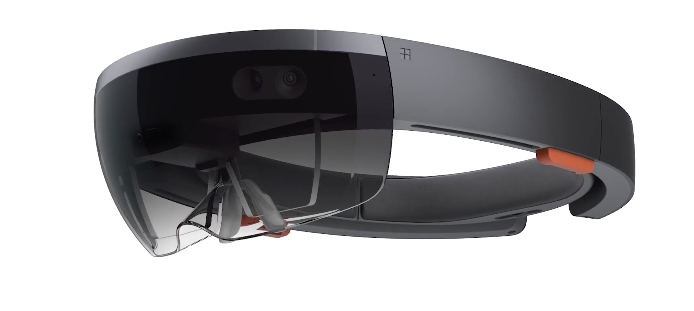
\includegraphics[width=70mm]{images/similarProducts/hololens} }}
    \qquad
    	\subfloat[Recon Jet\cite{reconJet}]{{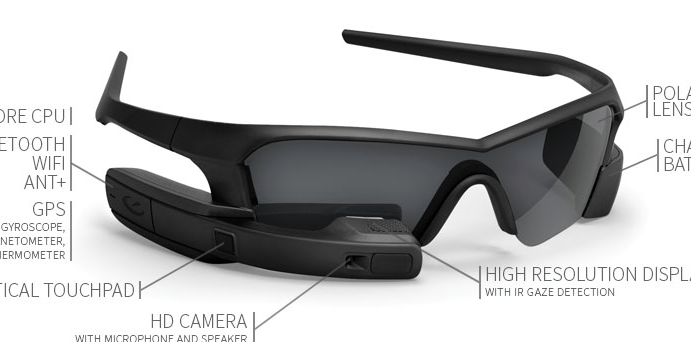
\includegraphics[width=70mm]{images/similarProducts/reconJet} }}
    \qquad
        \subfloat[GlassUp\cite{glassUpFeatures}]{{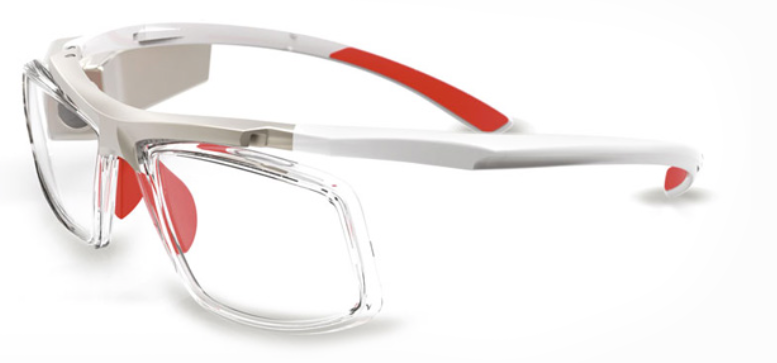
\includegraphics[width=70mm]{images/similarProducts/glassUp} }}
    \qquad
  	\subfloat[C Wear Interactive Glasses\cite{pennyProducts}]{{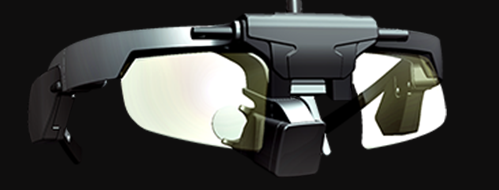
\includegraphics[width=70mm]{images/similarProducts/penny} }}
    \qquad
		\caption{Today there are many OHMD devices, either already on the market or under development. A more extensive list of devices can be found on wikipedia.\cite{ohmdWiki}}
		\label{imagesSimilarProducts}
	\end{figure}
\\
%\url{http://www.microsoft.com/microsoft-hololens/en-us}
%\url{http://www.searchenginejournal.com/google-glass-alternatives/67018/}
%\url{http://www.penny.se}